\chapter{GNU Radio OFDM Transceiver Implementation}\label{sec:TIOFDM}%
%
This chapter gives an introduction to an \gls{sdr} based GNU Radio OFDM transceiver implemented in our institute \cite{MZDARM}.
%
\begin{figure}[thb]
\centering
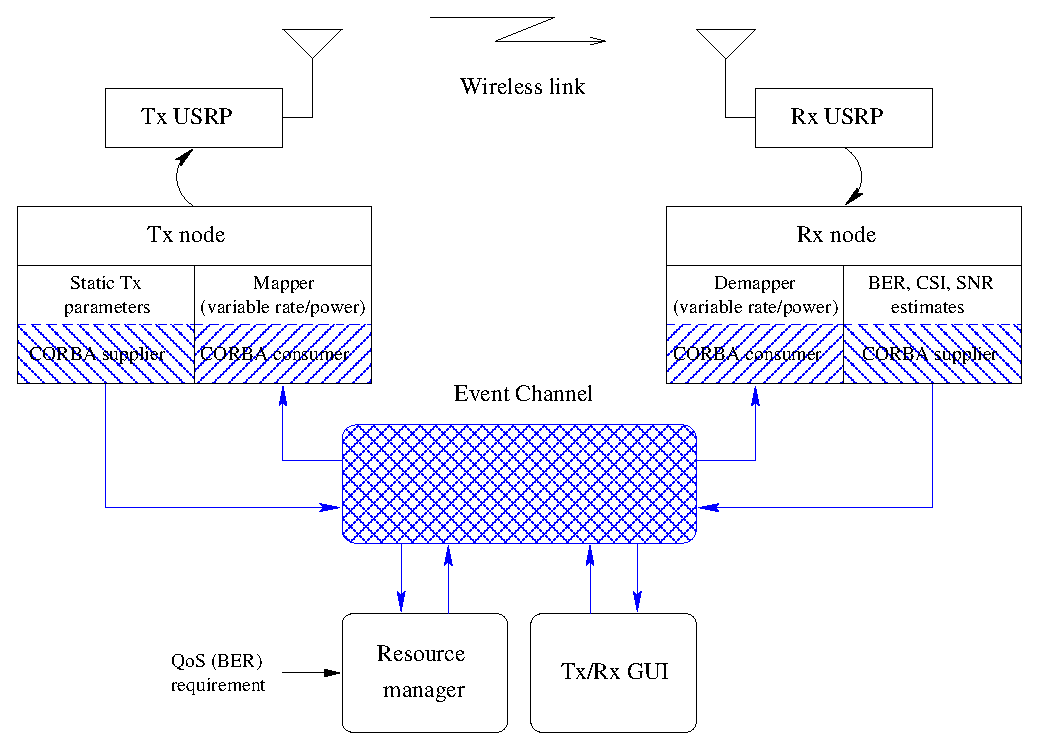
\includegraphics[width=0.54\linewidth]{grp_04.eps}
\caption{System overview\label{fig:sys_dig}}
\end{figure}
%
A system diagram of our \gls{ofdm} framework is shown in~\cref{fig:sys_dig}. Transmitter and receiver nodes are composed of a host commodity computer and general purpose \gls{rf} hardware, \gls{usrp}. The baseband signal processing at the host computers is implemented in the GNU~Radio framework.
%
\begin{figure}[ht]
\centering

 \begin{subfigure}[b]{0.56\linewidth}
 \centering
 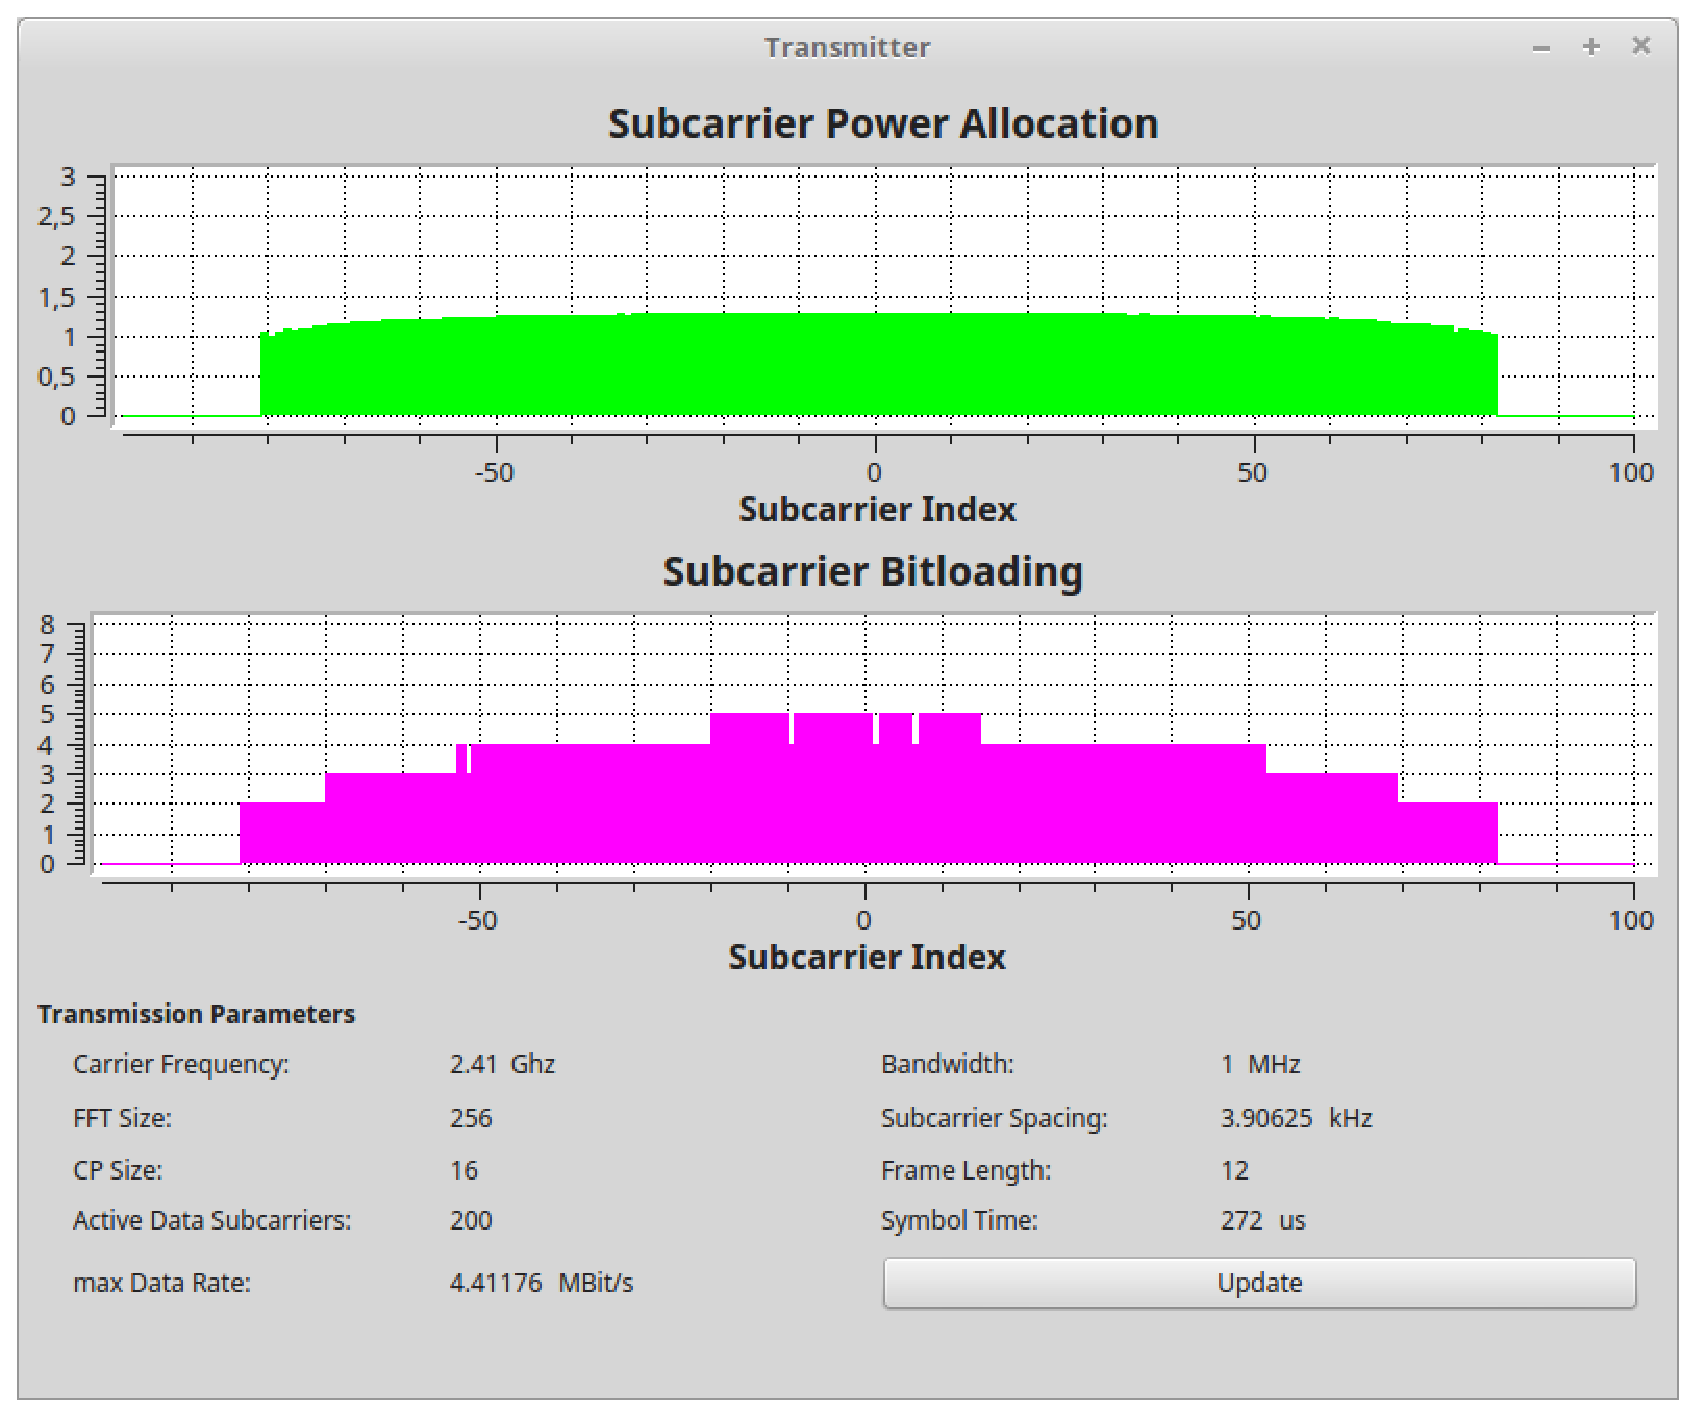
\includegraphics[width=\textwidth]{screenshot_tx.eps}
 \caption{The transmitter's GUI}\label{fig:txgui}
 \end{subfigure}

 \begin{subfigure}[b]{0.56\linewidth}
 \centering
 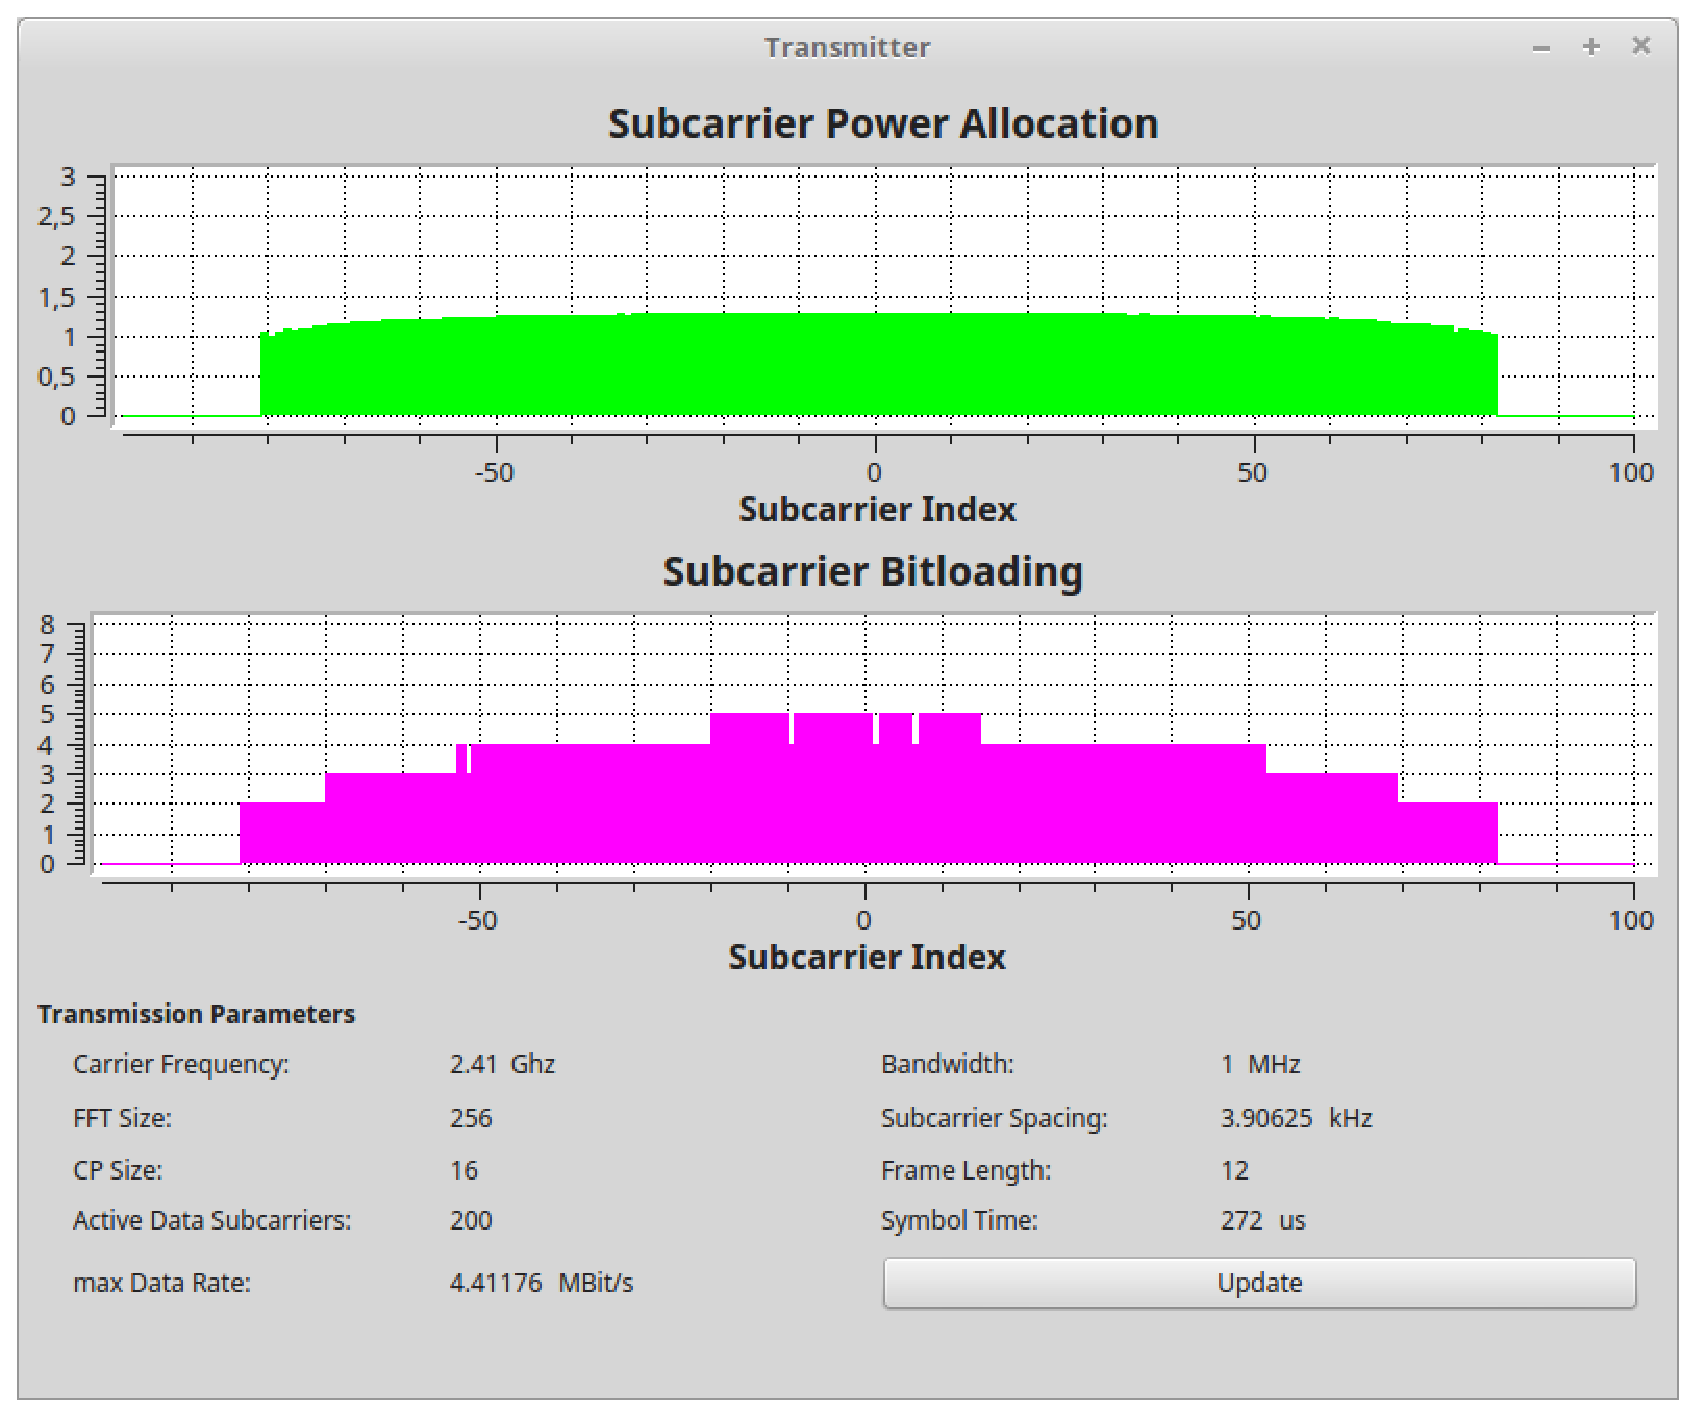
\includegraphics[width=0.665\linewidth]{screenshot_tx.eps}
 \caption{The receiver's GUI with interactive control interface}\label{fig:rxgui}
 \end{subfigure}
\caption{The framework's GUI with interactive control interface\label{fig:txrxgui}}
\end{figure}%
%
Within the framework, additional \gls{ofdm} specific GNU~Radio blocks are implemented, particularly at receiver's synchronization stage, since \gls{ofdm} systems are highly sensitive to \gls{to} and oscillators' mismatch between transmitter and receiver due to necessity for subchannel orthogonality, see Section~\ref{sec:sysimp}. The main adaptive and capacity achieving functionality is performed in blocks for adaptive mapping and demapping of various rates (taken from the set of available modulations given in Table~\ref{tab:tabtab}.1) and power levels across subchannels.
%
\begin{table}[tb]
\label{tab:tabtab}
\centering
{\scriptsize\begin{tabular}{| p{4.5cm}| p{5.5cm}|}\hline
Carrier frequency (\textbf{static})&$2400-2483$ MHz\\\hline
Bandwidth (\textbf{static})& Variable, up to $2$ MHz\\\hline
FFT length (\textbf{static})& $64-1024$\\\hline
Frame length (\textbf{static}) & Variable \\\hline
Modulations (\textbf{dynamic})&BPSK, QPSK, 8-PSK, 16-QAM, 32-QAM, 64-QAM, 128-QAM, 256-QAM\\\hline
Power (\textbf{dynamic})& Up to 20 mW\\\hline
\end{tabular} }%
\caption{OFDM symbol parameters}%
\end{table}%
%
Algorithms for estimation of link quality, expressed through average \gls{snr} and \gls{csi} over subchannels, are extensively studied and implemented at the receiver. Furthermore, in order to assess system performance, the receiver implementation contains blocks for \gls{ber} measurements.

The communication between transmitter and receiver node is organized as a reconfigurable continuous one-way transmission of OFDM symbol frames. As shown in Table~\ref{tab:tabtab}.1, the set of input configuration parameters can be divided into two classes. The set of \textbf{static parameters} containing \gls{fft}, number of subchannels, frame size, etc., is initialized at transmission start and is known to both nodes. The set of \textbf{dynamic parameters} which are reconfigurable at runtime includes total transmit power and allocated rate and power over subchannels.

The backbone of the system is realized over a local Ethernet network by a \CORBA\index{CORBA} \textbf{event service}~\cite{GNUCORBA}, a distributed communication model that allows an application to send an event that will be received by any number of objects located in different logical and/or physical entities, for more information on CORBA see~\cite{Mowbray,Orfali}. Estimated parameters that indicate link quality (average \gls{snr}, \gls{csi}, and \gls{ber}) and current static transmitter's parameters are supplied as \CORBA\index{CORBA} events to the \textbf{event channel} which allows other components (consumers) within the system to register their interests in events. The central control unit that determines optimal input transmission parameters for given requirements is called \textbf{resource manager}. Controlled by an interactive \gls{gui}\ it consumes supplied events forwarded from the \textbf{event channel}, performs allocation in an optimal manner, and supplies new transmission parameters, i.e., total transmit power and power/rate per subchannel, which are finally consumed by other components in the system.

The \GUI, facilitating the demonstration, is developed in Qt/\Cpp\ framework. The transmitter's \gls{gui} contains static transmission parameters and current allocation of rate and power over subchannels, as shown in ~\cref{fig:txgui}. Furthermore, the receiver's \GUI, given in ~\cref {fig:rxgui}, dynamically shows estimated channel parameters (average \gls{snr}, \gls{csi}, \gls{ber}) and contains an interactive interface for controlling allocation strategies and transmission parameters in the \textbf{resource manager}. 

The system can also run in simulation mode on a single PC, without the \RF \ interface (\gls{usrp} boards), where transmitter and receiver \glqq communicate\grqq\ over an artificial channel. A set of channel models available through \ITpp\ libraries \cite{GNUITPP} is ported to GNU~Radio framework in order to evaluate the system performance excluding hardware impairments.

Due to the high modularity and distributed nature of the system supported by a generalized interface, the dedicated \textbf{resource manager} can be easily reconfigured for different classes of given requirements and various sets of controllable parameters.
